\documentclass[12pt,a4paper]{article}
\usepackage[utf8]{inputenc}
\usepackage[T1]{fontenc}
\usepackage[italian]{babel}
\usepackage{geometry}
\usepackage{amsmath}
\usepackage{amssymb}
\usepackage{listings}
\usepackage{xcolor}
\usepackage{graphicx}
\usepackage{hyperref}
\usepackage{booktabs}
\usepackage{caption}
\usepackage{float}
\usepackage{parskip}
\usepackage{array}
\usepackage{tabularx}
\usepackage{tcolorbox}
\tcbuselibrary{listings,breakable,skins}
\usepackage{tikz}
\usetikzlibrary{arrows.meta, positioning, shapes.geometric, fit, calc}

\geometry{
  top=2.5cm, bottom=2.5cm,
  left=2.5cm, right=2.5cm
}

% Colori
\definecolor{codebg}{RGB}{248,248,248}
\definecolor{keywordcolor}{RGB}{0,0,180}
\definecolor{commentcolor}{RGB}{0,128,0}
\definecolor{stringcolor}{RGB}{163,21,21}
\definecolor{codeframe}{RGB}{180,180,180}

% Stile listings interno
\lstdefinestyle{python}{
  language=Python,
  basicstyle=\ttfamily\footnotesize,
  keywordstyle=\color{keywordcolor}\bfseries,
  commentstyle=\color{commentcolor}\itshape,
  stringstyle=\color{stringcolor},
  numberstyle=\tiny\color{gray},
  numbers=left,
  stepnumber=1,
  breaklines=true,
  breakatwhitespace=false,
  showstringspaces=false,
  tabsize=4,
  xleftmargin=1.5em,
  keepspaces=true,
  columns=flexible,
  frame=none,
  aboveskip=0pt,
  belowskip=0pt,
}
\lstset{style=python}

\hypersetup{
  colorlinks=true,
  linkcolor=blue!60!black,
  urlcolor=blue!60!black,
}

% Ambiente tcolorbox breakable per i listing Python
% uso: \begin{pylisting}[title={testo}]
\newtcblisting{pylisting}[1][]{
  listing only,
  enhanced,
  colback=codebg,
  colframe=codeframe,
  coltitle=black,
  fonttitle=\small\itshape,
  attach boxed title to top left={yshift=-2mm, xshift=4mm},
  boxed title style={colback=codebg, colframe=codeframe, boxrule=0.5pt},
  boxrule=0.5pt,
  arc=2pt,
  left=4pt, right=4pt, top=8pt, bottom=4pt,
  listing options={style=python},
  before upper={\vspace{-2pt}},
  #1
}

% Pagina del titolo personalizzata
\newcommand{\HRule}{\rule{\linewidth}{0.5mm}}

\begin{document}
\raggedbottom

% ============================================================
% FRONTESPIZIO
% ============================================================
\begin{titlepage}
  \centering
  \vspace*{1.5cm}

  {\Large\textbf{Università degli Studi di Torino}\\[0.3em]
  Corso di Laurea Magistrale in Informatica}

  \vspace{1cm}
  \HRule\\[0.4em]
  {\LARGE\textbf{Tecnologie del Linguaggio Naturale}}\\[0.3em]
  {\large Parte 2 -- Prof.\ Daniele Radicioni}\\[0.2em]
  \HRule

  \vspace{1.2cm}
  {\huge\textbf{Lab 4}}\\[0.5em]
  {\LARGE Modellazione del Linguaggio con N-grammi}\\[0.4em]
  {\large Confronto tra linguaggio dei social media e linguaggio letterario}

  \vspace{2cm}

  {\large\textbf{Gruppo di lavoro:}}\\[0.8em]
  \begin{tabular}{ll}
    \toprule
    \textbf{Studente}    & \textbf{Matricola} \\
    \midrule
    Alessandro Olivero   & 915069  \\
    Samuele Iudice       & 1235245 \\
    Andrea Franco        & 1226739 \\
    \bottomrule
  \end{tabular}

  \vspace{1.5cm}
  \begin{tabular}{ll}
    \textbf{Docente:}          & Prof.\ Daniele Radicioni \\[0.3em]
    \textbf{Anno Accademico:}  & 2025/2026 \\
  \end{tabular}

  \vfill
\end{titlepage}

\tableofcontents
\newpage

% ============================================================
\section{Introduzione}
% ============================================================

Questo laboratorio ha l'obiettivo di esplorare la \textbf{modellazione del linguaggio} tramite N-grammi, confrontando due domini linguistici molto diversi tra loro:

\begin{itemize}
  \item \textbf{Linguaggio Twitter}: messaggi brevi, informali, ricchi di slang, abbreviazioni ed emoji.
  \item \textbf{Linguaggio letterario}: testo formale tratto dal romanzo \textit{Emma} di Jane Austen (1816), caratterizzato da frasi lunghe e sintassi elaborata.
\end{itemize}

L'analisi copre i seguenti aspetti:
\begin{enumerate}
  \item Statistiche descrittive sui corpus (vocabolario, TTR, lunghezza frasi).
  \item Estrazione e analisi di bigrammi e trigrammi.
  \item Addestramento di modelli linguistici MLE e Laplace.
  \item Generazione automatica di testo.
  \item Classificazione di frasi tramite perplexity e log-likelihood.
\end{enumerate}

L'intero flusso sperimentale procede in tre fasi: i due corpus (Twitter e letterario) vengono puliti e tokenizzati separatamente, mantenendo ciascun tweet/frase come sequenza a sé (Sezione~\ref{sec:addestramento-lm} approfondito nella sezione 5); le sequenze vengono usate per addestrare due coppie di modelli n-gram (MLE e Laplace) indipendenti; dai modelli addestrati si diramano infine i tre utilizzi a valle discussi nel resto della relazione: generazione di testo, classificazione di dominio tramite perplexity e classificazione tramite log-likelihood.

% ============================================================
\section{Background Teorico}
% ============================================================

\subsection{N-grammi}

Un \textbf{N-gramma} è una sequenza contigua di $N$ token (parole) estratta da un testo. I casi più comuni sono:
\begin{itemize}
  \item \textbf{Unigramma} ($N=1$): singola parola.
  \item \textbf{Bigramma} ($N=2$): coppia di parole consecutive.
  \item \textbf{Trigramma} ($N=3$): tripletta di parole consecutive.
\end{itemize}

Gli N-grammi sono alla base dei \textbf{modelli linguistici statistici},stimanodo la probabilità di una parola dato il contesto delle $N{-}1$ parole precedenti.

\subsection{Modello MLE (Maximum Likelihood Estimation)}

Il modello MLE stima la probabilità condizionata alla frequenza relativa osservata nel corpus:

\[
  P_{\text{MLE}}(w_i \mid w_{i-1}) = \frac{C(w_{i-1},\, w_i)}{C(w_{i-1})}
\]

dove $C(\cdot)$ indica il conteggio nel corpus. Il problema principale del MLE è che assegna probabilità \textbf{zero} alle sequenze non viste nel training,è necessaria una singolaparola fuori dal vocabolario per rendere l'intera frase impossibile secondo il modello.

\subsection{Smoothing di Laplace (Add-1)}

Per ovviare al problema dello zero, lo \textbf{smoothing di Laplace} aggiunge 1 a ogni conteggio:

\[
  P_{\text{Laplace}}(w_i \mid w_{i-1}) = \frac{C(w_{i-1},\, w_i) + 1}{C(w_{i-1}) + |V|}
\]

dove $|V|$ è la dimensione del vocabolario. In questo modo nessuna sequenza ha probabilità nulla, al costo di ridistribuire parte della probabilità verso eventi non osservati.

\subsection{Perplexity}

La \textbf{perplexity} misura quanto un modello è ``sorpreso'' da un testo di test.

\[
  \text{PP}(W) = P(w_1 w_2 \cdots w_N)^{-\frac{1}{N}}
               = \left(\prod_{i=1}^{N} \frac{1}{P(w_i \mid w_{i-1})}\right)^{\frac{1}{N}}
\]

Minore è la perplexity, migliore è il modello per quel testo.

\subsection{Log-likelihood}

La \textbf{log-likelihood} di una sequenza misura quanto il modello ``conosce'' quel testo. Si calcola come somma dei logaritmi delle probabilità dati i singoli token:

\[
  \ell(W) = \sum_{i=1}^{N} \log P(w_i \mid w_{i-1})
\]

Il valore è sempre $\leq 0$: più è vicino a zero (meno negativo), meglio il modello descrive il testo. Rispetto alla perplexity è numericamente più stabile ed è diretta da usare come classificatore: si assegna un testo al dominio che gli assegna log-likelihood più alta.

\subsection{Type-Token Ratio (TTR)}

Il \textbf{TTR} misura la ricchezza lessicale di un testo:

\[
  \text{TTR} = \frac{|\text{Types}|}{|\text{Tokens}|}
\]

dove \textit{Types} sono le parole uniche e \textit{Tokens} sono tutte le occorrenze. Valori alti indicano vocabolario vario; valori bassi indicano ripetitività.

% ============================================================
\section{Dataset e Pre-elaborazione}
% ============================================================

\subsection{Dataset}

\begin{itemize}
  \item \textbf{Twitter}: corpus \texttt{twitter\_samples} di NLTK, composto da 5\,000 tweet positivi e 5\,000 tweet negativi (10\,000 tweet in totale).
  \item \textbf{Letterario}: testo integrale di \textit{Emma} di Jane Austen (1816), disponibile nel corpus \texttt{gutenberg} di NLTK.
\end{itemize}

\subsection{Pipeline di pulizia}

I due corpus richiedono trattamenti diversi a causa della natura del linguaggio.

\begin{pylisting}[title={Pulizia dei tweet e del testo letterario}]
def pulisci_tweet(testo):
    testo = re.sub(r'http\S+', '', testo)          # rimuove URL
    testo = re.sub(r'@\w+', '', testo)             # rimuove menzioni
    testo = re.sub(r'#', '', testo)                # rimuove simbolo hashtag
    testo = re.sub(r'[^a-zA-Z\s]', '', testo)     # solo lettere
    testo = testo.lower().strip()
    return testo

def pulisci_letterario(testo):
    testo = re.sub(r'[^a-zA-Z\s]', '', testo)
    testo = testo.lower().strip()
    return testo
\end{pylisting}

Per i tweet si rimuovono URL, menzioni e hashtag prima di normalizzare il testo. Per il testo letterario si rimuovono solo i caratteri non alfabetici, mantenendo la struttura originale.

% ============================================================
\section{Analisi Statistica dei Corpus}
% ============================================================

\subsection{Tokenizzazione e vocabolario}

\begin{pylisting}[title={Tokenizzazione e calcolo del vocabolario}]
tokens_tweet = word_tokenize(testo_tweet_unito)
tokens_lett  = word_tokenize(testo_lett_pulito)

vocab_tweet_set = set(tokens_tweet)
vocab_lett_set  = set(tokens_lett)
\end{pylisting}

\begin{table}[H]
  \centering
  \caption{Statistiche descrittive dei corpus}
  \begin{tabular}{lrr}
    \toprule
    \textbf{Statistica} & \textbf{Twitter} & \textbf{Letterario} \\
    \midrule
    Token totali           & 94\,706 & 158\,267 \\
    Parole uniche (types)  & 12\,024 & 9\,305   \\
    TTR grezzo$^{*}$       & 0.1270  & 0.0588   \\
    Lunghezza media frase  & 16.0 token & 25.6 token \\
    \bottomrule
  \end{tabular}
  \\[0.3em]
  {\footnotesize $^{*}$Calcolato sull'intero corpus di ciascun dominio: non è un confronto valido, perché il TTR scende all'aumentare dei token. Il confronto corretto, su campioni di uguale dimensione, è in Sezione~11.1.}
\end{table}

Le parole uniche riflettono la dimensione del vocabolario di ciascun corpus così com'è, mentre il testo letterario ha frasi molto più lunghe in media. Il TTR grezzo qui sopra non è direttamente confrontabile tra i due domini (Sezione~11.1 presenta il confronto corretto).

\subsection{Rimozione delle stopwords e analisi dei bigrammi}

\begin{pylisting}[title={Rimozione stopwords e calcolo bigrammi/trigrammi}]
stop = set(stopwords.words('english'))

tokens_tweet_filtrati = [t for t in tokens_tweet if t not in stop]
tokens_lett_filtrati  = [t for t in tokens_lett  if t not in stop]

bi_tweet_filtrati = Counter(ngrams(tokens_tweet_filtrati, 2))
bi_lett_filtrati  = Counter(ngrams(tokens_lett_filtrati,  2))
\end{pylisting}

Rimuovendo le stopwords emergono i bigrammi semanticamente significativi di ciascun dominio:
\begin{itemize}
  \item \textbf{Twitter}: bigrammi legati a emozioni (\textit{feel good}, \textit{love much}), auguri (\textit{happy birthday}) e relazioni (\textit{miss much}).
  \item \textbf{Letterario}: bigrammi tipici del romanzo vittoriano (\textit{mr knightley}, \textit{miss woodhouse}, \textit{emma thought}).
\end{itemize}

% ============================================================
\section{Addestramento dei Modelli Linguistici}
\label{sec:addestramento-lm}
% ============================================================

\subsection{Preparazione e fitting}

NLTK fornisce \texttt{padded\_everygram\_pipeline}, che aggiunge automaticamente i token di inizio (\texttt{<s>}) e fine (\texttt{</s>}) frase e genera tutti gli N-grammi fino a $n$. Ogni tweet e ogni frase del romanzo viene passato come sequenza a sé stante, in modo che il padding (e quindi i bigrammi generati) non attraversi il confine tra un tweet/frase e il successivo:

\begin{pylisting}[title={Addestramento modelli MLE e Laplace per bigrammi ($n=2$)}]
n = 2

sequenze_tweet = [word_tokenize(t) for t in tweets_puliti]
frasi_lett_raw = sent_tokenize(testo_letterario_raw)
sequenze_lett  = [word_tokenize(pulisci_letterario(f)) for f in frasi_lett_raw]
sequenze_lett  = [s for s in sequenze_lett if s]

# Modelli MLE: per generazione e probabilita' condizionali
train_tw_mle, vocab_tw_mle = padded_everygram_pipeline(n, sequenze_tweet)
modello_tweet = MLE(n)
modello_tweet.fit(train_tw_mle, vocab_tw_mle)

train_lt_mle, vocab_lt_mle = padded_everygram_pipeline(n, sequenze_lett)
modello_lett = MLE(n)
modello_lett.fit(train_lt_mle, vocab_lt_mle)

# Modelli Laplace: per perplexity (gestisce parole mai viste)
train_tw_lp, vocab_tw_lp = padded_everygram_pipeline(n, sequenze_tweet)
modello_tweet_lp = Laplace(n)
modello_tweet_lp.fit(train_tw_lp, vocab_tw_lp)

train_lt_lp, vocab_lt_lp = padded_everygram_pipeline(n, sequenze_lett)
modello_lett_lp = Laplace(n)
modello_lett_lp.fit(train_lt_lp, vocab_lt_lp)
\end{pylisting}

Si addestrano due varianti per ciascun corpus:
\begin{itemize}
  \item \textbf{MLE}: usato per la generazione di testo e il calcolo delle probabilità condizionali.
  \item \textbf{Laplace}: usato per la perplexity, poiché MLE assegna probabilità 0 a parole mai viste, rendendo la perplexity infinita.
\end{itemize}

\textbf{Nota su una correzione di correttezza}: in una prima versione, tutti i tweet (o tutte le frasi del romanzo) venivano concatenati in un'unica sequenza prima di essere passati a \texttt{padded\_everygram\_pipeline}. Questo produceva un solo \texttt{<s>}/\texttt{</s>} per l'intero corpus, e generava bigrammi spuri a cavallo tra la fine di un tweet e l'inizio del successivo (una relazione che nella realtà non esiste). Passare una sequenza per ogni tweet/frase risolve il problema.

\subsection{Probabilità condizionali}

\begin{pylisting}[title={Calcolo probabilità condizionali con MLE}]
# Modello Twitter
print(modello_tweet.score('love',  ['i']))    # P('love' | 'i')
print(modello_tweet.score('happy', ['so']))   # P('happy' | 'so')

# Modello Letterario
print(modello_lett.score('mr',   ['said']))   # P('mr' | 'said')
print(modello_lett.score('been', ['had']))    # P('been' | 'had')
\end{pylisting}

Le probabilità condizionali riflettono il registro linguistico: il modello Twitter assegna alta probabilità a \textit{love} dopo \textit{i}, mentre il letterario assegna alta probabilità a \textit{mr} dopo \textit{said} e a \textit{been} dopo \textit{had}, strutture tipiche della prosa ottocentesca.

% ============================================================
\section{Generazione di Testo}
% ============================================================

\begin{pylisting}[title={Generazione di testo con filtraggio degli artefatti}]
def genera_testo(modello, n_parole=30):
    testo_raw = modello.generate(n_parole, random_seed=42)

    testo_filtrato = []
    for token in testo_raw:
        # scarta token speciali del padding
        if token in ['<s>', '</s>', '<UNK>']:
            continue
        # scarta lettere singole (artefatti), tranne 'i' e 'a'
        if len(token) == 1 and token not in ['i', 'a']:
            continue
        testo_filtrato.append(token)

    return ' '.join(testo_filtrato)

# Esempi di output
print(genera_testo(modello_tweet, 40))   # stile Twitter
print(genera_testo(modello_lett,  40))   # stile letterario
\end{pylisting}

Il metodo \texttt{generate()} campiona parola per parola usando le probabilità del bigramma. I token \texttt{<s>}, \texttt{</s>} e \texttt{<UNK>} sono artefatti del padding e vengono rimossi. Le lettere singole (diverse da \textit{i} e \textit{a}) sono artefatti di tokenizzazione e vengono anch'esse filtrate.

\textbf{Esempi di testo generato} (seed=42, 40 parole):
\begin{itemize}
  \item \textit{Stile Twitter}: frasi brevi, emotivamente cariche, con ripetizioni tipiche dei social.
  \item \textit{Stile letterario}: frasi più lunghe, con lessico formale e costruzioni sintattiche elaborate tipiche di Austen.
\end{itemize}

% ============================================================
\section{Perplexity Cross-Domain}
% ============================================================

\subsection{Configurazione dell'esperimento}

L'idea è usare la perplexity come classificatore: dato un testo, il modello che gli assegna \textbf{perplexity più bassa} è quello del dominio di appartenenza.

Si usano 8 frasi di test (4 da Twitter, 4 letterarie) e si calcola la perplexity con entrambi i modelli Laplaciani. La Funzione \texttt{perplexity()} di NLTK si aspetta in input una sequenza di n-grammi (non i token grezzi), quindi le frasi vengono prima riportate in bigrammi con padding tramite \texttt{pad\_both\_ends}. Poiché i vocabolari hanno dimensioni molto diverse, il verdetto si basa sulla perplexity normalizzata per la dimensione del vocabolario:

\begin{pylisting}[title={Classificazione tramite perplexity normalizzata}]
def calcola_perplexity(modello, tokens, n=2):
    ngr = list(ngrams(pad_both_ends(tokens, n=n), n))
    return modello.perplexity(ngr)

for nome, frase in frasi_test.items():
    tokens_frase = word_tokenize(frase)
    pp_tw   = calcola_perplexity(modello_tweet_lp, tokens_frase, n)
    pp_lett = calcola_perplexity(modello_lett_lp, tokens_frase, n)

    # Normalizza per la dimensione del vocabolario
    pp_tw_n   = pp_tw   / len(modello_tweet_lp.vocab)
    pp_lett_n = pp_lett / len(modello_lett_lp.vocab)

    verdetto_atteso = "TW" if nome.startswith("tw") else "LT"
    verdetto        = "TW" if pp_tw_n < pp_lett_n else "LT"
    corretto        = "corretto" if verdetto == verdetto_atteso else "errato"
\end{pylisting}

\begin{table}[H]
  \centering
  \caption{Perplexity diLaplace (non normalizzata) sulle 8 frasi di test}
  \begin{tabular}{lrrc}
    \toprule
    \textbf{Frase} & \textbf{PP Twitter} & \textbf{PP Letterario} & \textbf{Verdetto} \\
    \midrule
    tw\_pos\_1 & 128.1  & 538.7  & TW \checkmark \\
    tw\_pos\_2 & 1425.3 & 3434.1 & TW \checkmark \\
    tw\_neg\_1 & 235.7  & 2151.0 & TW \checkmark \\
    tw\_neg\_2 & 577.8  & 1375.3 & TW \checkmark \\
    lett\_1    & 6321.1 & 290.1  & LT \checkmark \\
    lett\_2    & 797.7  & 159.3  & LT \checkmark \\
    lett\_3    & 3821.2 & 442.0  & LT \checkmark \\
    lett\_4    & 2605.8 & 126.2  & LT \checkmark \\
    \bottomrule
  \end{tabular}
\end{table}

Con la perplexity calcolata correttamente sui bigrammi, il verdetto (basato sui valori normalizzati) è corretto per tutte le 8 frasi: \textbf{accuratezza 8/8 = 100\%}.

\subsection{Limiti della perplexity come classificatore}

Su questo specifico set di frasi la perplexity normalizzata raggiunge il 100\% di accuratezza, tanto quanto la log-likelihood (Sezione~8): i due domini sono linguisticamente così distanti che entrambi i metodi separano correttamente ogni frase di test. Il vantaggio della log-likelihood non è quindi visibile in questo esperimento, ma resta valido sul piano teorico: la normalizzazione per $|V|$ usata per la perplexity è una correzione empirica, non una pratica standard, mentre la log-likelihood confronta direttamente due modelli sullo stesso testo senza bisogno di questo aggiustamento ad hoc.

% ============================================================
\section{Classificatore con Log-Likelihood}
% ============================================================

\begin{pylisting}[title={Calcolo della log-likelihood di una sequenza}]
def log_likelihood(modello, tokens):
    # Log-prob. media per token. Richiede Laplace: con MLE un bigramma
    # mai visto avrebbe prob. 0 e il floor sotto dominerebbe la somma.
    score = 0.0
    for i in range(1, len(tokens)):
        contesto = [tokens[i-1]]
        parola   = tokens[i]
        prob = modello.score(parola, contesto)
        if prob > 0:
            score += math.log(prob)
        else:
            score += math.log(1e-10)  # floor, quasi mai attivo
    return score / (len(tokens) - 1)

def classifica_loglik(testo, mod_tw, mod_lt):
    tokens  = word_tokenize(testo.lower())
    ll_tw   = log_likelihood(mod_tw,   tokens)
    ll_lett = log_likelihood(mod_lt,   tokens)
    # vince il modello con log-likelihood piu' alta
    verdetto = "TWITTER" if ll_tw > ll_lett else "LETTERARIO"
    return verdetto, ll_tw, ll_lett

for testo in testi_classificare:
    classifica_loglik(testo, modello_tweet_lp, modello_lett_lp)  # Laplace, non MLE
\end{pylisting}

\textbf{Perché i modelli Laplace e la media per token.} Il classificatore
usa i modelli Laplace, non MLE. Con MLE un bigramma mai visto in training
ha probabilità esattamente $0$: scatterebbe il floor ($\log 10^{-10}
\approx -23$), che pesa quanto $7$--$8$ bigrammi ordinari e finirebbe per
decidere da solo il verdetto — il classificatore conterebbe i bigrammi
sconosciuti invece di confrontare le verosimiglianze. Con Laplace la
probabilità non è mai nulla e il floor non si attiva mai. Lo score è
inoltre diviso per il numero di transizioni: una log-likelihood media per
token è confrontabile anche fra frasi di lunghezza diversa.

Il classificatore assegna il testo al modello con log-likelihood più alta (meno negativa). Rispetto alla perplexity normalizzata, questo approccio ha alcuni vantaggi metodologici:
\begin{itemize}
  \item Non richiede di dividere per la dimensione del vocabolario per rendere i due modelli confrontabili.
  \item Un floor di $10^{-10}$ (invece di $P=0$) evita i valori $-\infty$ sui bigrammi mai visti, pur restando un caso limite che con Laplace non si attiva quasi mai.
\end{itemize}

\begin{table}[H]
  \centering
  \caption{Log-likelihood media per token (modelli Laplace) sulle 8 frasi di test}
  \small
  \begin{tabular}{>{\raggedright\arraybackslash}p{6.8cm}rrl}
    \toprule
    \textbf{Frase} & \textbf{LL Twitter} & \textbf{LL Letterario} & \textbf{Verdetto} \\
    \midrule
    i love you so much thank you                 & $-5.289$ & $-7.138$ & TWITTER \\
    she had been very well disposed towards him   & $-9.205$ & $-6.143$ & LETTERARIO \\
    i miss you so much cant stop thinking         & $-6.476$ & $-8.280$ & TWITTER \\
    it was a very good thing to have done         & $-6.828$ & $-5.110$ & LETTERARIO \\
    happy birthday love you so much               & $-5.622$ & $-7.727$ & TWITTER \\
    she was not a woman of many words             & $-8.288$ & $-6.323$ & LETTERARIO \\
    i cant stop smiling so happy                  & $-7.662$ & $-8.890$ & TWITTER \\
    mr knightley had always been very fond of her & $-9.062$ & $-5.882$ & LETTERARIO \\
    \bottomrule
  \end{tabular}
\end{table}

Tutti gli 8 verdetti coincidono con il dominio atteso: \textbf{accuratezza 8/8 = 100\%}, in linea con quanto ottenuto dalla perplexity normalizzata (Sezione~7). Si noti che questo set di frasi è diverso (per quanto in parte sovrapposto) da quello usato in Sezione~7 per la perplexity.

% ============================================================
\section{MLE vs.\ Laplace: confronto diretto}
% ============================================================

\begin{pylisting}[title={Confronto MLE e Laplace su parola mai vista}]
parola_rara = "xyzword"
print(modello_tweet.score(parola_rara, ['i']))     # MLE    -> 0.0
print(modello_tweet_lp.score(parola_rara, ['i']))  # Laplace -> valore > 0

frase_rara = word_tokenize("i xyzword lol")
pp_mle = calcola_perplexity(modello_tweet,    frase_rara, n)  # MLE -> inf
pp_lap = calcola_perplexity(modello_tweet_lp, frase_rara, n)
\end{pylisting}

\begin{table}[H]
  \centering
  \caption{Confronto MLE vs.\ Laplace su frase con parola mai vista}
  \begin{tabular}{lcc}
    \toprule
    \textbf{Metrica}              & \textbf{MLE}     & \textbf{Laplace} \\
    \midrule
    $P(\text{xyzword} \mid i)$    & $0.000000$       & $0.000065$       \\
    Perplexity su frase rara      & $\infty$         & $1111.48$        \\
    \bottomrule
  \end{tabular}
\end{table}

Il MLE è inutilizzabile per calcolare la perplexity su frasi con parole fuori vocabolario (basta una singola parola ignota per rendere l'intera frase impossibile secondo il modello, con perplexity infinita), mentre Laplace garantisce sempre un valore finito.

% ============================================================
\section{Confronto $n=1, 2, 3$}
% ============================================================

Tutti e tre i modelli sono addestrati solo sul corpus Twitter (\texttt{sequenze\_tweet}), e la stessa frase viene valutata sia in-dominio (Twitter) sia fuori dominio (letteraria):

\begin{pylisting}[title={Confronto della perplexity al variare di $n$}]
frase_tw = word_tokenize("i love you so much thank you")
frase_lt = word_tokenize("she had been very well disposed")

for n_test in [1, 2, 3]:
    tr_tmp, voc_tmp = padded_everygram_pipeline(n_test, sequenze_tweet)
    mod_tmp = Laplace(n_test)
    mod_tmp.fit(tr_tmp, voc_tmp)

    pp_tw = calcola_perplexity(mod_tmp, frase_tw, n_test)
    pp_lt = calcola_perplexity(mod_tmp, frase_lt, n_test)
    print(f"n={n_test}: PP Twitter={pp_tw:.2f}, PP Letterario={pp_lt:.2f}")
\end{pylisting}

\begin{table}[H]
  \centering
  \caption{Perplexity Laplace al variare di $n$ (modelli addestrati solo su Twitter)}
  \begin{tabular}{lrr}
    \toprule
    \textbf{$n$} & \textbf{PP frase Twitter} & \textbf{PP frase Letteraria} \\
    \midrule
    1 & 124.04 & 1727.63  \\
    2 & 128.14 & 8059.42  \\
    3 & 307.20 & 10003.72 \\
    \bottomrule
  \end{tabular}
\end{table}

All'aumentare di $n$:
\begin{itemize}
  \item La perplexity aumenta per \emph{entrambe} le frasi, non solo per quella fuori dominio: con $n$ maggiore lo smoothing di Laplace deve distribuire probabilità su uno spazio di n-grammi molto più grande ($|V|^n$), e la maggior parte non è mai stata osservata nel training. Questo effetto di \textbf{data sparsity} penalizza anche la frase in-dominio.
  \item L'aumento è però molto più marcato per la frase letteraria (fuori dominio): il divario tra le due perplexity si allarga passando da $n=1$ a $n=2$, segno che il modello sta imparando dipendenze sempre più specifiche del corpus Twitter, che la frase letteraria non rispetta.
  \item Questo mostra un compromesso pratico: aumentare $n$ rende il modello più specifico al proprio dominio (utile per distinguere i due stili), ma anche più fragile per data sparsity quando applicato a un corpus di addestramento di dimensioni moderate.
\end{itemize}

% ============================================================
\section{Analisi Linguistica Comparata}
% ============================================================

\subsection{Type-Token Ratio}

Il TTR non è confrontabile calcolandolo sull'intero corpus di ciascun dominio: è una quantità che \emph{scende} strutturalmente all'aumentare del numero di token (le parole nuove si esauriscono via via che il testo prosegue), quindi confrontare il TTR di $\sim$95\,000 token di tweet con quello di $\sim$158\,000 token di \textit{Emma} misura soprattutto quale corpus è più piccolo, non quale sia lessicalmente più vario. Il TTR va quindi calcolato su campioni di uguale dimensione:

\begin{pylisting}[title={Calcolo del TTR su campioni di uguale dimensione}]
N = min(len(tokens_tweet), len(tokens_lett))
ttr_tweet = len(set(tokens_tweet[:N])) / N
ttr_lett  = len(set(tokens_lett[:N]))  / N
\end{pylisting}

Su un campione di $N = 94\,706$ token (la dimensione dell'intero corpus Twitter, il più piccolo dei due) si ottiene $\text{TTR}_{\text{Twitter}} = 0.1270$ e $\text{TTR}_{\text{Letterario}} = 0.0719$. Twitter mantiene un TTR più alto anche a parità di token campionati (nonostante il divario si riduca rispetto al confronto non corretto, che dava $0.1270$ vs.\ $0.0588$): il vocabolario resta eterogeneo per la presenza di slang, hashtag, nomi propri e abbreviazioni, mentre il testo letterario, anche su un campione della stessa dimensione, usa un vocabolario relativamente più ristretto e ricorrente.

\subsection{Lunghezza media delle frasi}

\begin{pylisting}[title={Calcolo della lunghezza media delle frasi}]
lung_tw  = [len(word_tokenize(t)) for t in tweets_raw]
frasi_lt = sent_tokenize(testo_letterario_raw)
lung_lt  = [len(word_tokenize(f)) for f in frasi_lt]

media_tw = sum(lung_tw) / len(lung_tw)
media_lt = sum(lung_lt) / len(lung_lt)
\end{pylisting}

Le frasi letterarie sono circa il doppio più lunghe dei tweet: il romanzo di Austen è ricco di subordinate e costruzioni relative, mentre i tweet tendono a essere telegrafici.

% ============================================================
\section{Risultati e Discussione}
% ============================================================

La Figura~\ref{fig:confronto-risultati} raccoglie in un unico pannello i risultati chiave discussi nelle sezioni precedenti: i bigrammi più frequenti nei due domini (Sezione~4.2), il confronto diretto di log-likelihood sulle quattro frasi di test (Sezione~8) e le metriche linguistiche strutturali (TTR e lunghezza media, Sezione~11).

\begin{figure}[H]
\centering
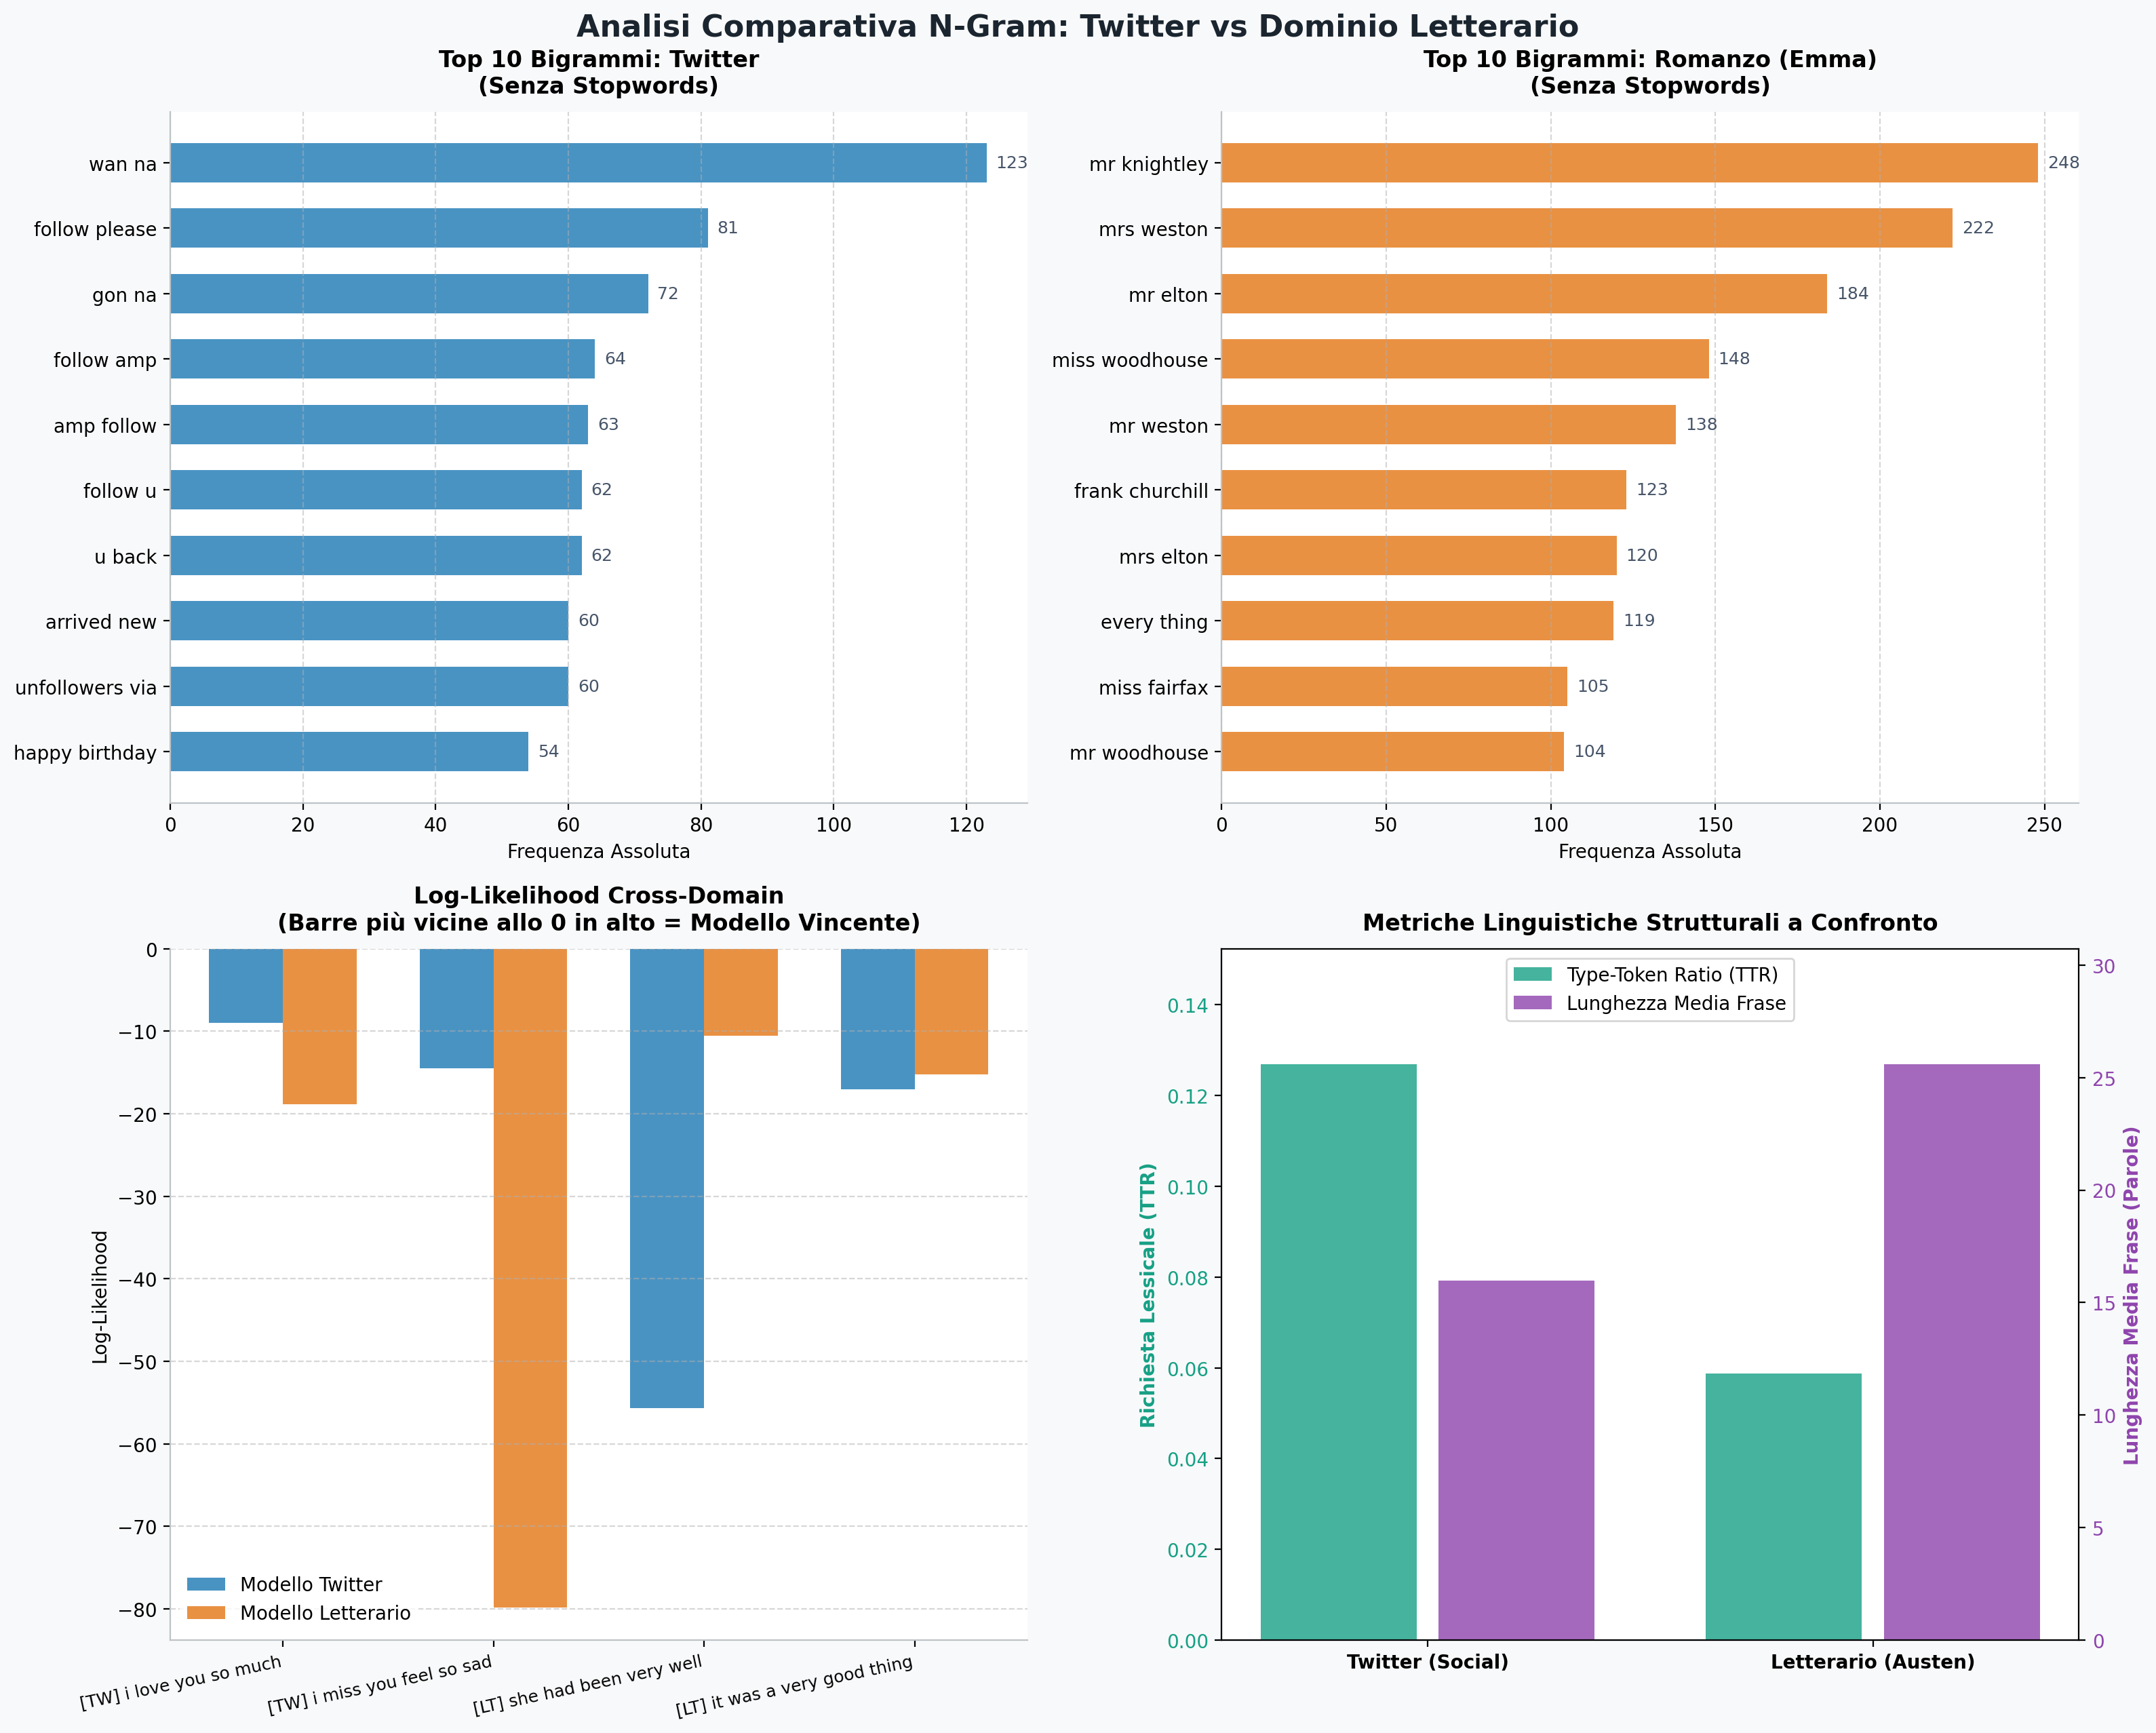
\includegraphics[width=\textwidth]{confronto_risultati_laboratorio.png}
\caption{Riepilogo visivo: top-10 bigrammi per dominio (senza stopword), log-likelihood cross-domain sulle quattro frasi di test, e confronto di TTR e lunghezza media frase.}
\label{fig:confronto-risultati}
\end{figure}

\subsection{Perché entrambi i classificatori raggiungono il 100\%}

Sia la perplexity normalizzata (Sezione~7) sia la log-likelihood (Sezione~8) classificano correttamente \emph{tutte} le frasi di test. Il motivo è strutturale: il vocabolario di Twitter (slang, forme contratte, hashtag) e quello di Austen (registro ottocentesco, nomi propri come \textit{Mr.\ Knightley}) si sovrappongono solo in un nucleo comune di parole funzionali, per cui una frase di un dominio contiene quasi sempre bigrammi mai osservati nel modello dell'altro — con Laplace questo si traduce in una perplexity nettamente peggiore per il modello ``sbagliato''.

Questo spiega anche perché il vantaggio teorico della log-likelihood (non richiede la normalizzazione ad hoc per $|V|$, Sezione~7.2) non si traduca qui in un'accuratezza misurabilmente superiore: il compito è troppo facile per discriminare fra i due metodi. Un test più severo userebbe frasi di confine (es.\ testo giornalistico, a metà fra i due registri) invece di frasi nettamente appartenenti a un dominio.

\subsection{Il ruolo dello smoothing: non solo evitare probabilità zero}

Il confronto MLE vs.\ Laplace (Sezione~9) mostra che lo smoothing non è solo un accorgimento anti-crash, ma cambia concretamente l'output: su una parola mai vista, MLE assegna probabilità $0$ e perplexity $\infty$ (inutilizzabile per classificare o confrontare frasi), mentre Laplace assegna una probabilità piccola ma finita ($6.5 \times 10^{-5}$) e una perplexity finita ($1111.48$). Senza smoothing, l'intera pipeline di valutazione delle Sezioni~7 e~10 sarebbe stata impossibile su dati reali, dove le parole fuori vocabolario sono la norma.

\subsection{L'ordine $n$ non aiuta linearmente: il costo della sparsity}

Il confronto fra $n=1,2,3$ (Sezione~10, Tabella~5) mostra che la perplexity \emph{aumenta} con $n$ per entrambe le frasi, non solo per quella fuori dominio: la PP Twitter passa da $124.04$ a $307.20$ ($n{=}1\to3$), perché lo spazio degli n-grammi cresce come $|V|^n$ mentre i dati di training restano fissi (data sparsity). L'effetto è però molto più marcato fuori dominio: la PP letteraria passa da $1727.63$ a $10003.72$ (fattore $\sim5.8\times$ contro $\sim2.5\times$ per Twitter). Aumentare $n$ non rende quindi un modello ``migliore'' in assoluto, ma più specifico al proprio dominio — utile per un classificatore, ma rischioso per generazione o autocompletamento, dove il testo in input non sempre coincide con lo stile del training.

\subsection{Sintesi tabellare}

\begin{table}[H]
  \centering
  \caption{Riepilogo delle caratteristiche dei due domini}
  \begin{tabular}{lcc}
    \toprule
    \textbf{Caratteristica}  & \textbf{Twitter}   & \textbf{Letterario} \\
    \midrule
    Dataset                  & 10\,000 tweet      & \textit{Emma}, Austen (1816) \\
    TTR (campioni pari)      & alto (0.1270)      & basso (0.0719)      \\
    Lunghezza media frase    & 16.0 token         & 25.6 token          \\
    Bigrammi tipici          & emozioni, auguri   & titoli, azioni      \\
    Smoothing consigliato    & Laplace            & Laplace             \\
    \bottomrule
  \end{tabular}
\end{table}

\subsection{Osservazioni principali}

\begin{enumerate}
  \item \textbf{I modelli N-gram riflettono lo stile del corpus}: il testo generato da ciascun modello è chiaramente riconoscibile come appartenente al dominio di addestramento.

  \item \textbf{Entrambi i classificatori raggiungono il 100\% di accuratezza} (Sezione~12.1): un risultato dovuto alla forte distanza lessicale fra i due domini più che a un vantaggio specifico di un metodo sull'altro.

  \item \textbf{Laplace è indispensabile per la robustezza} (Sezione~12.2): MLE è ottimo per stimare probabilità su dati visti, ma non può gestire frasi di test con parole nuove.

  \item \textbf{$n=2$ è un buon compromesso}: cattura dipendenze locali senza soffrire troppo di sparsity, a differenza di $n=3$.

  \item \textbf{Twitter è linguisticamente più vario ma meno strutturato}: TTR più alto anche a parità di token campionati, frasi brevi, bigrammi emotivi. Austen ha TTR più basso ma struttura sintattica ricca.
\end{enumerate}

% ============================================================
\section{Conclusioni}
% ============================================================

Il laboratorio ha dimostrato come i modelli linguistici basati su N-grammi siano in grado di catturare differenze stilistiche significative tra due domini molto distanti. Il modello addestrato su Twitter genera testo informale e ripetitivo, mentre quello addestrato su Austen produce frasi più formali e articolate.

Sia la perplexity normalizzata sia la log-likelihood classificano correttamente il 100\% delle frasi di test: la distanza linguistica tra i due domini è tale da rendere il compito facile per entrambi i metodi. La log-likelihood resta preferibile sul piano metodologico perché confronta i due modelli senza bisogno di una normalizzazione ad hoc per la dimensione del vocabolario. Le tecniche di smoothing (in particolare Laplace) restano comunque essenziali per rendere i modelli applicabili a testi reali che contengono inevitabilmente parole fuori vocabolario.

% ============================================================
\section{Dichiarazione sui Contributi di IA}
% ============================================================

Per questo laboratorio ci siamo appoggiati anche a uno strumento di intelligenza artificiale generativa (Claude, Anthropic), usato come supporto puntuale durante lo sviluppo e non come autore del lavoro. Qualche esempio concreto di come lo abbiamo usato:

\begin{itemize}
  \item \textbf{Snellimento dei commenti nel codice}: molti commenti erano troppo lunghi o ripetevano quanto già scritto nel testo; li abbiamo resi più diretti (es.\ perché serve addestrare un modello Laplace separato da MLE, o cosa misura esattamente la perplexity normalizzata per vocabolario).
  \item \textbf{Individuazione e correzione di due bug metodologici}: \texttt{perplexity()} di NLTK si aspetta in input n-grammi, non token grezzi (passandole i token grezzi calcola probabilità su singoli caratteri anziché su parole), e i modelli venivano addestrati su un'unica sequenza per l'intero corpus invece che una per ciascun tweet/frase, generando bigrammi spuri a cavallo tra un tweet e il successivo. Dopo la correzione abbiamo rilanciato lo script e aggiornato tutte le tabelle di perplexity con i valori reali (Sezioni~7, 9, 10).
  \item \textbf{Verifica di piccoli dettagli di correttezza}: rilettura del codice per controllare che pipeline di preprocessing, addestramento e valutazione fossero coerenti tra i due domini (Twitter e letterario).
  \item \textbf{Correzione di un'incoerenza tra codice e docstring}: il classificatore a log-likelihood veniva chiamato con i modelli MLE anziché Laplace, in contraddizione con la docstring della funzione; con MLE un bigramma mai visto attiva un floor artificiale ($\log 10^{-10}$) che di fatto decide la classificazione al posto della verosimiglianza reale. Abbiamo anche normalizzato lo score per la lunghezza della frase, per confrontare correttamente frasi di lunghezza diversa.
  \item \textbf{Correzione del confronto TTR}: il Type-Token Ratio calcolato sull'intero corpus non era confrontabile tra i due domini (dipende dalla dimensione del corpus); ricalcolato su campioni di uguale dimensione (Sezione~11.1).
\end{itemize}

L'impostazione del lavoro, le scelte metodologiche, l'interpretazione critica dei risultati e la stesura della relazione restano nostre.

\end{document}
